% This is samplepaper.tex, a sample chapter demonstrating the
% LLNCS macro package for Springer Computer Science proceedings;
% Version 2.20 of 2017/10/04
%
\documentclass[runningheads]{llncs}
%
\usepackage{graphicx}
\usepackage{hyperref}
\renewcommand\UrlFont{\color{blue}\rmfamily}
\setlength{\parskip}{0pt}
\raggedbottom

\usepackage{amsmath}
\usepackage{csquotes}
\usepackage{paralist}
\usepackage{booktabs}
\usepackage{mathptmx}
\usepackage{pgfplots}
\pgfplotsset{compat=1.8}
\usepackage{subfigure}

\begin{document}
%
\title{Towards an efficient Prediction Model\\ of Malaria Cases in Senegal}
%
%\titlerunning{Abbreviated paper title}
% If the paper title is too long for the running head, you can set
% an abbreviated paper title here
%
\author{Ousseynou Mbaye \and Mouhamadou Lamine Ba \\ Gaoussou Camara \and Alassane Sy}
%
\authorrunning{Ousseynou Mbaye \and M. Lamine Ba \and Gaoussou Camara \and Alassane Sy}
% First names are abbreviated in the running head.
% If there are more than two authors, 'et al.' is used.
%
\institute{Universit\'e Alioune Diop de Bambey, Bambey, Senegal\\
\email{firstmidlle.last@uadb.edu.sn}
%\email{ousseynou.mbaye@uadb.edu.sn}\\
%\email{mouhamadoulamine.ba@uadb.edu.sn}\\
%\email{gaoussou.camara@uadb.edu.sn}\\
%\email{alassane.sy@uadb.edu.sn}
}
%
\maketitle              % typeset the header of the contribution
%
\begin{abstract}
Among  the most deadly disease in the world, Malaria remains a real flail in Sub-saharan Africa 
in particular. In countries like Senegal, such a situation is acute due to the lack of high quality
healthcare services and well-formed staffs able to perform accurate diagnosis of diseases that patients suffer from. 
This calls for the need of finding automated tools to help medical actors in their decision making process.
In this paper, we present first steps towards an efficient way to automatically diagnosis Malaria occurence or not 
based on patient signs and symptoms, and the outcome from the quick diagnosis test. Our prediction approach is built
on the logistic regression function. First expermients on a real world patient dataset, as well as a semi-synthetic dataset,
show promising performance results regarding the effectiveness of the proposed approach.
 
\keywords{Malaria  \and Diagnosis \and Data imputation \and Prediction Model.}
\end{abstract}
%
%
% Introduction
\section{Introduction}\label{intro}
Malaria is one amongst the most deadly disease in the world, especially in sub-saharan Africa countries such as Senegal.
Malaria is caused by parasitic single-celled microorganisms belonging to the Plasmodium group; it is an infectious
disease which is transmitted to human being through bites from infected female Anopheles mosquitoes. Someone who suffers
from  Malaria may present symptoms that typically include fever, tiredness, vomiting, and headaches. In its severe form,
the disease can cause yellow skin, seizures, coma or death.

\subsubsection{Studied problem and motivations.}
According to the last report \cite{Wh17}  about the propagation of Malaria disease around the world, published in November 2017 by the World international Health Organization (WHO in short),
 216 millions of cases have been reported in 2016. As a result, the number of cases has significantly increased when compared to the 211 millions of reported Malaria patients in 2016.
As for the number of death due to Malaria, it does not decrease between 2016 and 2017 (446.000 vs. 445.000) despite the huge effort made by governements
and non-governmental organization to improve healthcare services and the awareness strategies, especially in critical areas. 
When analyzing the statistics above in details, one can easily notice that the burden of the Africa region of the World 
international Health Organization is colossal. Indeed, 90\% of Malaria cases and 90\% of deaths due to the disease were located in this area in 2016.
More specifically, 80\% of the burden in terms of morbidity is distributed in fifteen countries, all located in Sub-saharan Africa except India. This demonstrates
that Malaria is a real flail in Sub-saharan Africa states and Senegal is not spared at all. We investigate in this study an efficient approach to predict, using machine learning, the occurence 
or not of Malaria when a patient has to be diagnosed. Given the patient signs and symptoms, as well as the result from the quick diagnosis test, our solution should be to 
automatically tell if she suffers from Malaria or not with a high accuracy.

Malaria is an acute problem in Senegal  due mainly to the lack of high quality healthcare services and well-formed
staffs able to perform accurate diagnosis of diseases that patients suffer from. Over the past years, the government with 
the help of international organizations have tried to eradicate Malaria by implementing various proactive and reactive solutions 
to fill the gap in terms of services and human resources. However, the mortality rate is still very high, e.g. in underserved areas,
areas without required healthcare needs, uneducated people, population with low income, etc. Most of these deaths cases are reported to be caused by inaccurate diagnosis, sometimes 
incomplete leading to a bad prediction of the exact type of Malaria.
On the other hand, Malaria occurence or complication can often occur during  popular events (for instance religious events such as the Grand Magal of Touba \cite{So17})
which gather thousands of persons from everywhere in the country during a short time period. During those popular events, non-permanent medical points are set in order
to assist and treat ill persons; the staff in a given health point might be formed sometimes by only volunteers without advanced medical skills. Each of these medical 
points might receive and treat hundreds of patients each day with some of them potentially suffering from Malaria. 
This appeals for the need of finding automated tools to help medical actors in their decision making process, and thereby to improve provided 
healthcare services.   

\subsubsection{Proposed diagnosis approach.}
In this paper we present first steps towards an efficient manner to automatically diagnosis Malaria occurence or not based on patient signs and symptoms,
and the outcome from the quick diagnosis test. We define our diagnosis task as a classical binary classification problem by considering two classes: \textquote{Malaria} and \textquote{not-Malaria}.
Given a patient data, our main goal is to properly find to which class the patient belongs. To solve this classification problem we rely on machine learning and use the logistic regression
function as the basis of our prediction approach. Machine learning has been largely used in several domains (e.g. Health Informatics  \cite{Du13}) for various purposes whereas logistic regression has demonstrated its efficiency when dealing with a binary classification problem. 
 
As an application scenario, we focus on predicting Malaria cases in Senegal. At this end, we use  a large volume of patient record dataset collected during the most popular religious event in Senegal from the different installed health points, namely more than twenty points that deadly receive hundreds of patients.
As an immediate result of this work, we introduce a data preparation pipeline in order to 
\begin{inparaenum}[(i)]
\item explore the dataset for profiling purpose;
\item only retain records related to Malaria;
\item clean and transform attributes, as well data values, into the extracted Malaria dataset; and 
\item impute missing values (there were lot of missing values in the collected health dataset as reported in Section\ref{data_prep}).
\end{inparaenum}
Such a data preparation pipeline has been realized using \emph{OpenRefine} (formely Google Refine) to perform various cleaning and profiling tasks on our raw atient dataset and \emph{missForest}, a robust
 algorithm for imputing  missing data of diverses types; see Section \ref{data_prep} for more details. 
Expermients on the real world patient dataset, augmenting with a semi-synthetic dataset, show promising performance results regarding the effectiveness of the proposed approach.

\subsubsection{Paper organization.}The remaining of the paper is organized as follows. We summarize the related work on data imputation and binary classification methods in Section \ref{related_work}.
In Section \ref{data_prep} we introduce a data preparation pipeline on the raw collected patient records for the prediction phase. 
We then present our prediction model for Malaria cases in Section \ref{prediction_model}.
Experiments and performance analysis  on the collected real-world dataset, as well as a semi-synthetic dataset,  are detailled in Section \ref{experimentation} before we conclude in Section \ref{conclusion}. 


% Related work
\section{Related work}\label{related_work}
In this section, we summarize the sate-of-the-art research on Malaria in general, and in particular the
use of machine learning techniques to tackle the various aspects related to one of the 
major healthcare problems worldwide which is Malaria.

% Studies on Malaria
As it is well-known, Malaria is caused by the bite of the female Anopheles, the most dangerous of which
is Plasmodium falciparum. Many early works have been consequently focused on the study of the evolution and
the distribution of the responsible mosquito, mainly with the goal to detect or diagnosis the severity of the 
disease given an infected patient \cite{Fe03,Al09}. Recent research on Malaria have largely adopted machine learning
and showed its ability to solve various aspects of the disease. Most of these machine learning based techniques are 
based on the analysis of blood data obtained from high-definition microscopic screenshots as in \cite{Ku18}. The authors
in \cite{Ku18} propose an unsupervised learning algorithm that detects and determines the types of infected blood cells.
Used prediction approach consists of quantifying the amount of plasmodium parasites in a blood smear. In the same research intuition
of harnessing blood, the Jordan-Elman neural network classifier introduced in \cite{Ha15}, on the other hand, to quickly determine the occurrence 
of Malaria and its severity level as well: the neural network analyzes the features of the blood data of the patients.  
Still using ML, DIAZ et al. have proposed in \cite{Dia09} a semi-supervised algorithm enable to quantify and classify the 
erythrocytes infected by Malaria parasistes through microscopic images. The orginiality of this work comes from its usability
even in the presence of thin blood drandruff infected by falciparum Plasmodium for the quantification and the classificationi tasks.
Besides blood data, sign and symptom records were also used to study Malaria with ML methods. Indeed, decision trees based approach
has been proposed in Nigeria \cite{Ug10} to predict the occurrence of Malaria given diagnostic data. However a decision tree suffers 
from various limitations as a classifier. Indeed it can easily overfit or can be extremely sensitive to small pertubations in data for instance.
Even though we both rely on signs and symptoms, the prediction model in \cite{Ug10} differs from ours on numerous facets: our model is built upon
logistic regression and is trained using also inputs from the quick diagnosis test. In addition, we apply our method in the context of patients living in Senegal. 
An example of previous work that has used logistic regression is that of Farida et al. in \cite{Ad10}. The logistic regression is exploited
there for the selection of features in order to construct stable decision trees. The decision trees are then used to predict the severity
criteria of Malaria in the context of Afghanistan. 


In the same line of works applying machine learning, in \cite{Pr17}, Pranav et al. propose Malaria likelihood prediction model built on a deep reinforcement learning (RL) agent. 
Such a RL predicts the probability of a patient testing positive for Malaria using answers from questions about their household. In 
the presented approach the authors have also dealt with the problem of determining the right question to ask next as well as the length of the survey, dynamically.
Moreover, statistically enhanced rule-based classification model to diagnose malaria has been proposed in \cite{Bb16}. A corresponding prototype 
which incorporates the rules and statistical models have been implemented; the main goal of the study was to develop a statistical 
prototype to perform clinical diagnosis of malaria given its adverse effects on the overall healthcare, yet its treatment remains 
very expensive for the majority of the patients to afford.

To the best of our knowledge this is the first work in Senegal that attempts to provide a prediction model for identifying 
the occurrence of Malaria given patient data.  


% Data Preparation
\section{Data Preparation}\label{data_prep}
In this section, we detail the data preparation pipeline followed to obtain a proper Malaria dataset for the prediction phase.
We start by presenting the used data cleaning and normalization techniques.


% data cleaning and normalization
\subsection{Data cleaning and normalization}
In order to set up an efficient prediction model for Malaria cases in Senegal, we have relied on a real-world patient dataset
for validation purposes. The dataset was extracted in 2016 during the Grand Magal of Touba \cite{So17}. 
An estimated 4-5 million individuals gather each year in the holy city of Touba, Senegal during the Grand Magal religious pilgrimage.
Several health points are set during this religious event; every point dairly receives hundreds of patients, some of them 
suffering from Malaria. The patient data we are using here have been manually recordered from these points in registers as no electronic
health management system does exist.  

In detail, the dataset consists of thousands of patient records having each 16 attributes. Some of these
attributes (also knwon as features) comprise personal data about the patient, but also patient signs and symptoms
reported by the doctor who took in charge the patient. The other attributes describe clinical data such as information about the final diagnosis
of the doctor (the disease that the patient suffers from), the income of the quick diagnosis test, and the status (i.e. admission, 
dead or put under observation) of the patient. For privacy concerns and some restrictions in data use, we have disregarded personal data about
the patient during this work. Due to the fact that patient records have been collected manually in registers, we have noticed many inconsistencies 
such as misspellings, same attribute values with different writings (e.g., \textquote{DIARRHEE INFECTIEUSE} and \textquote{INFECTIEUSE DIARRHE}),
 and multi-valued attributes (e.g. sign and symptom reported values). We use OpenRefine \cite{Ku16,openRefine} to first clean and then normalize values in the patient dataset.

OpenRefine (formerly called Google Refine) is a powerful open source tool that allows researchers or scientists to accomplish the data wrangling activity, i.e. 
working with messy data: cleaning it; transforming it from one format into another; and extending it with Web services and external data.    
We used the following methods provided by OpenRefine to pre-treat our raw dataset.

\begin{itemize}
\item \textbf{Text filter function:} text filter enables to expore attribute values, clean them, and to identify those that may have many variants. 
\item \textbf{Transform functions:} OpenRefine provides two different Transform functions: preset transformations for resolving trivial formatting issues like trimming whitespaces
and advanced transformations based on the OpenRefine Expression Language (GREL) to normalize data in batch or split them. This second class of transformations is very useful, especially when the 
number of piece of data values to normalize is very important (doing the same task manually would be time-consuming and prone to errors). For instance, GREL allows to use a simple
regular expression all variants of a symptom in the Symptom column.  
\item \textbf{Cluster and edit function:} Clustering option in OpenRefine also provides users with methods to merge and normalize variations across the dataset. The power of clustering
is that it is able to automatically detect small data variations which follow a certain pattern.  
\end{itemize}

As for the special case of multi-valued attributes such as symptom and diagnosis columns in our raw dataset, we splitted them into multiple values in distinct columns.
Indeed, in the raw dataset information like the symptoms a given patient suffer from were stored in a single column, separated with the special character '+', e.g. \textquote{DOULEUR ARTICULAIRE}
+ \textquote{DOULEUR PELVIENNE} + \textquote{VOMISSEMENTS}.


After this step of data cleaning and normalization, we have proceeded to the extraction of Malaria features.

% Extraction of Malaria features
\subsection{Extraction of Malaria features}
To properly study Malaria, one needs to have a patient dataset with the main features of the disease. 
Unfortunately, some of these Malaria features were not explicitly specified in our raw dataset.
As a result, we have inferred twelve new attributes that better describe the signs and symptoms 
of Malaria according to experts in the health domain. Those new attributes are : \emph{lack of appetite},
\emph{tiredness}, \emph{fever}, \emph{cephalalgia}, \emph{nausea}, \emph{arthralgia}, 
\emph{digestive disorders}, \emph{dizziness}, \emph{chill}, \emph{myalgia}, \emph{diarrhea}, and \emph{abdominal pain}.  
We have then added the new attributes in our dataset and transformed this latter accordingly by filling the value of each new attribute based on the 
list of reported signs and symptoms for every patient.

A medical diagnostic is the results the analysis of the reported signs and symptoms; in general such a diagnostic is further confirmed by a medical test.
Since our raw dataset does not contain only information about patients from Malaria, yielding to records with various diagnostics. For the purposes of 
our study, we replaced any diagnostic that is not Malaria by the class \textquote{Not-Malaria}. At this step of our data preparaton pipeline, we came 
up with a patient dataset that contains required Malaria features. However, our Malaria was not yet complete and ready because of values missingness.
As a last step, we have completed our dataset by using a robust data imputation approach.

% Data Imputation Approach

\subsection{Missing Data Imputation}
As shown in Table \ref{table-missing}, we observed many missing values in our dataset, affecting the majority of the data attributes. Such missing values
should not be ignored as data completeness and quality are very important when dealing with a prediction problem; this could negatively impact the accuracy
of our prediction and should be treat appropriately. One has to note that machine learning relies on complete dataset.
The sources and types of missing values can be various \cite{Al18}. In our context, missingness is \emph{not
completely random} and can be due to an incomplete knowledge of the patient data, the fact that the medical staff do not specify a attribute value when it is
not observed, or a difficulty for the patients to properly describe some piece of information (e.g. related to the signs or symptoms of their diseases) at the
diagnostic time. Since they might have a certain relationship between attribute values for the same patient, or even a correlation between patient records, we 
decide to solve our problem of missing values by using imputation algorithms instead of choosing arbitrary values or removing records with missing values.  

Data imputation is often used in the machine learning field when dealing with missing information. Many algorithms have been proposed in the literature \cite{Si14,Al18},
depending on the nature of the missingness or the type of data. MissForest \cite{Ste12} has been proved to be efficient at the presence of various types (e.g. numerical data,
string, categorical data, ect.) of data simultaneously as in our case.
The algorithm missForest relies on Random Forest, a non-parametric prediction method that is able to to deal with mixed-type data and allows for intreactive and non-linear regression effects.
Such a imputation algorithm aims at handling any type of input dataset by minimizing (when possible) assumption about the structural apsects of the data. Given an input dataset, missForest
solves the missing data problem using an iterative imputation scheme by training a Random Forest on observed values in a first step, followed by predicting the missing values 
and then proceeding iteratively until convergence. 

We have applied missForest on our Malaria patient dataset by using its open-source Python implementation \cite{MF_python}. We shall study and prove in Section \ref{experimentation} the accuracy of
the prediction made by the algorithm with the hep of the normalized root mean squared error metric.  

% table of the number of missing values per attribute
\begin{table}[!ht]
\centering
\begin{tabular}{cc}
\textbf{Attribute name} & \textbf{\#missing\_values}\\
\toprule
Lack of appetite &    21068 \\
digestive disorders & 21062 \\
Loss of weight &   21017 \\
Arthragia &     20940\\
Chill &      20925\\
Nausea &     20874\\
Myalgia &    20870\\
Tiredness&   20713 \\
Diarrhea &     20481\\
Vomit &        20051 \\
Abdominal pain &  19770 \\
Dizziness &       19628 \\
Fever &        18245 \\
Temperature &     17636 \\
Arterial pressure &    16924 \\
Cephalalgia &       15370 \\
Diagnostic  &     2875 \\
Quick diagnostic test &  76 \\
\bottomrule
\end{tabular}
\vspace*{.5cm}
\caption{The number of missing values per attribute}\label{table-missing}
\end{table} 


% Prediction Model
\section{Prediction Model}\label{prediction_model}
To learn from labelled patient dataset and be able to properly predict 
the occurence or not of Malaria given a new patient, we harness the logistic 
regression function as our \emph{classifier}. 
In this section, we briefy recall the basic of the logistic regression function
and how it can act as a binary classifier. We start by introducing the binary 
classification problem we have to solve in the study.

% binary classification problem for Malaria
\subsection{Binary classification problem}
Let us assume two given classes of Malaria diagnostic: \emph{Malaria} and \emph{Not-Malaria}.
We also consider \textsc{P} and \textsc{C} as respectively the set of patients and a prediction model.
A patient \emph{p} in \textsc{P} is defined by a set of pairs $(a_1, v_1), (a_2, v_2), \ldots, (a_n, v_n)$
where $a_i$ and $v_i$, for each $1\leq i\leq n$, respectively corresponds to a given Malaria feature and its associated value defined
as follows.
\begin{equation}
v_i = \left\{
\begin{array}{rl}
1 &\text{if $a_i$ is observed} \\
0 &\text{otherwise} \\
\end{array}
\right.
\end{equation}

\begin{definition}{(Our prediction problem)}
We define our binary classification problem for the prediction of the occurrence
or not of Malaria on a given patient dataset as a mapping \textsc{C} of every patient p in \textsc{P} 
to one and only one class in \{Malaria, Not-Malaria\}. Formally, we present such a mapping as \textsc{C}: \textsc{P} $\mapsto$ \{Malaria, Not-Malaria\}.
\end{definition}


We define and use  \textsc{C} with the help of the logistic regression for the specific purpose of our study. 
% Logistic regession function
\subsection{Logistic regression}
The logistic regression (a.k.a the logit function) is a statistical model used in the machine learning domain for binary classification \cite{Ch14}.
In its basic form, it is based on a logistic function to model a binary dependent variable \cite{Ho00,Sa14}.
As an input, the logistic regression  takes qualitative or/and ordinal predictive variables (e.g. the presence
or not of fever given a patient) in order to measure the probability of the outcome (e.g. the occurrence or not of the Malaria) 
by using the \emph{Sigmoid function}. Figure \ref{sigmoid_curve} shows the shape of the curve of the Sigmoid function. 

% The curve of the logistic regression
\begin{figure}[ht]
\centering
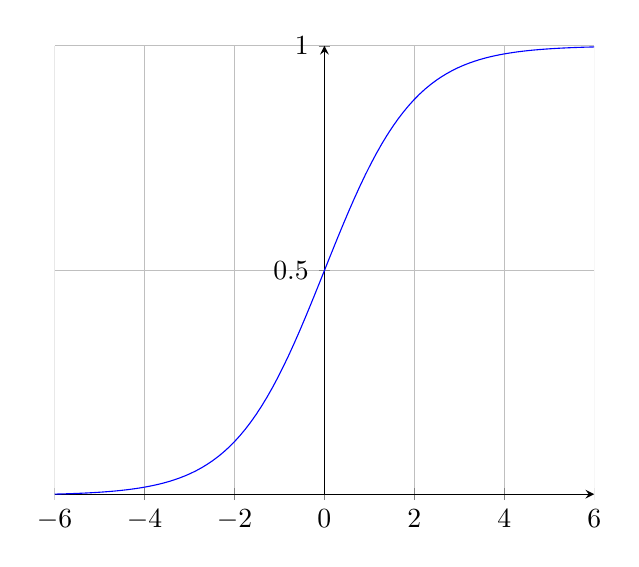
\begin{tikzpicture}
    \begin{axis}%
    [
        grid=major,     
        xmin=-6,
        xmax=6,
        axis x line=bottom,
        ytick={0,.5,1},
        ymax=1,
        axis y line=middle,
    ]
        \addplot%
        [
            blue,%
            mark=none,
            samples=100,
            domain=-6:6,
        ]
        (x,{1/(1+exp(-x))});
    \end{axis}
\end{tikzpicture}
\caption{The curve of the Sigmoid function}\label{sigmoid_curve}
\end{figure}

The logistic regression is one of the most used multi-valued models in epidemiology \cite{Am02,Pr05} (i.e. the study of the incidence,
 distribution, and possible control of diseases and other factors relating to health issues that can affect groups of population).
In such a context, the variable to explain is often the occurrence or not of an event like a disease and the explanatory 
variables, i.e. the features, are those that highly impact the occurrence of this event, i.e. variables assessing the exposure to a 
risk factor or a protective factor, or a variable representing the confusion factor.
The main interest of using logistic regression is its ability to quantify the strength of the relationship between each explicative 
variable and the variable to explain, given the other variables integrated to the model \cite{Am02}. 

% formal definition of the logistic model
\subsubsection{Formal definition  of our regression  model.}
Let us assume that \textsc{Y} represents the variable we are trying to explain in this study, i.e. the variable which models the occurrence or not of Malaria and whose 
two classes \emph{Malaria} and \emph{Not-Malaria} are respectively denoted by \textsc{M+} and \textsc{M-}. 

In the special case of only one explicative variable \emph{a} (which case corresponds to a simple regression), formally
the model is written as follows.

\begin{equation}
\textsc{Pr}(\textsc{M+} ~|~ \emph{a}) = \frac{e^{\alpha + \beta\times \emph{a} }}{1 + e^{\alpha + \beta\times \emph{a} }}
\label{simple_regression}
\end{equation}
where the coefficients $\alpha$ abd $\beta$ are the parameters of the model.

\textsc{Pr}(\textsc{M+} ~$|$~ \emph{a}) measures the probability of the occurrence of Malaria if the variable \emph{a} is observed.
Figure \ref{sigmoid_curve} represents the corresponding logistic function \emph{f(a)}. Again, the main interest of this function
lies in the simplicity of reaching an estimation of an odds ratio (OR) which measures the strength of the association between the 
disease \textsc{M} and an exposure variable in a regression analysis. Indeed if the value exposure variable is either $0$ (the variable is not observed)
or $1$ (the variable is observed) as in our setting, the model enables to obtain after some simplifications OR = $e^{\beta}$. The coefficient $\beta$ 
of the exposure variable in the logistic model is then the logarithmic of the odds ratio which measures the relationship between the explanatory variable 
(sign or symptom) and the disease (Malaria); this eases the analysis of the results of the logistic regression. 

An extension of the simple regression to a model with multiple variables (a.k.a multiple regression) is straightforward as we show with the formula below.

\begin{equation}
\textsc{Pr}(\textsc{M+} ~|~ \emph{$a_1$},\emph{$a_2$}, \ldots, \emph{$a_n$}) = \frac{e^{\alpha + \sum_{i=1}^{n} \beta_i \times \emph{$a_i$} }}{1 + e^{\alpha + \sum_{i=1}^{n} \beta_i \times \emph{$a_i$} }}
\label{multiple_regression}
\end{equation} 
where to every variable \emph{$a_i$} is associated a coefficient $\beta_i$. The corresponding odds ratio OR$_i$, quantifying the relationship between \emph{$a_i$} and \textsc{M+} is equal to $e^{\beta_i}$.

% Selection of the final model
\subsubsection{Model optimization.}
The question that generally raises when using a multiple regression approach is how to select the minimum set of variables amongst the \emph{$a_i$}'s that better explain the variable \textsc{Y}.  
Several optimization strategies are possible to obtain the best final prediction model which takes into account the maximum of information
while restricting as much as possible the number of explanotory variables in order to ease the analysis of the results:
\emph{stepwise descendant} and \emph{stepwise ascendant} are the most used approaches. Both approaches apply an iterative 
regression by first including in the model the variable that presents the best determination coefficient and then by adding the
variable which improves this coefficient and so on for stepwise ascendant. For stepwise decendant, the entire set of variables are considered at the beginning and variables are gradually excluded
from the model, depending on those which do not significantly improve the determination coefficient.

We next present the results of our prediction of Malaria cases by using our logistic regression model above on real-world patient datasets.    


% Experimentation and Results
\section{Experimentation and results}\label{experimentations}
We detail and analyze in the section the results of the experimentation we performed using the six ML algorithms presented in Section \ref{ml_algorithms} over the two real datasets described in Section \ref{datasets}. We start by presenting our experimentation setting.

% experimentation setting
\subsection{Experimentation Setting}
In this section data is available for applying classification algorithm. After model creation from training data, classification operation is performed on test data. 
All the performed tests have been done in the same machine and the same operating system. To test the performance of our six chosen ML algorithms, we relied on their Python implementations available through the scikit-learn library. Scikit-learn is an open source simple and efficient tool for predictive data analysis that implements most of the existing ML algorithms

Then some of the most important performance evaluation measures like accuracy, precision, sensitivity, specificity, F-measure and area under ROC curve are evaluated and compared. 
For the details about the description of each parameter of ML we refer to the official documentation of the implementation of these algorithms in scikit-learn7. Concerning the segmentation of both datasets for the training of our ML algorithms and their testing we have considered the stratified-5-fold cross-validation in classification model construction and efficiency evaluation. This method is very useful to handle data with an unbalanced class distribution, increases the validation of classification and prevents from random and invalid results.


% Results of the experiments
\subsection{Results of the experiments}

This section presents the results of the experimentation on each real dataset for each of the six classifiers. 
\subsubsection{Decision Tree}

Table 1  below shows the performance measures (precision, recall, F measure and precision) of the results of our Decision Tree classifier after experimentation on all our datasets. The observation shows that the best scores of our classifier are achieved on the datasets DT1, DT3 and DT5 which are 97.04\%, 80.86\% and 83.41\% respectively. Also AUC (Area Under the Curve) values are higher for these same datasets which are 0.78, 0.86 and 0.76 respectively. However, we note that the sensitivity values are higher than the specificity values on the datasets DT1, DT3  and DT5 whereas they are substantially lower than thoses of datasets DT2 and DT4. This means that DT is more inclined to predict as well whether a given patient has malaria or he doesn’t, on the datasets DT2, DT3 and DT4, while our classifier on the datasets DT1 and DT5 our classifier is only efficient in predicting whether a given patient has malaria. This same trend is observed on the F-scores which higher values varying between 0.91 and 0.98 on the datasets DT1, DT3 and DT5.

% Decision Tree
\begin{table}[!ht]
\centering
\begin{tabular}{*{7}{c}l r}
  \toprule
  \textbf{Datasets} & \textbf{Precision} & \textbf{Recall} & \textbf{F1-score}&\textbf{AUC} &\textbf{Score}&\textbf{Specificity}\\
   \midrule
  DT1 &0.97  & 1   & 0.98 & 0.78 & 97.04 & 0.05 \\
  DT2 & 0.59 &0.48 &0.48  &0.64  &63.01  &0.80\\
  DT3 &0.89  &0.85 &0.87  &0.86  &80.86  &0.69\\
  DT4 &0.68  &0.57 &0.62  &0.70  &65.60  &0.74\\
  DT5 &0.99  &0.84 &0.91  &0.76  &83.41  &0.58\\

  
    \bottomrule
\end{tabular}
\caption{Performances measures of DT over all datasets}\label{perf-measure-dt1}
\end{table}
\subsubsection{Random Forest}
The performance of the random forest varied throughout the study depending on the dataset, although overall it performed well as shown in Table 2. Notice that best accuracy are achieved by random forest classifier on the datasets DT1, DT2 and DT5 which are respectively 97.13\%, 80.86\% and 78.35\%. In contrast with the results obtained with the DT classifier, the Sensivity values are higher than specificity values on datasets DT1 and DT5 whereas the inverse is noticed on the dataset DT3. At the same time we note that these values are roughly identical on the datasets DT3 and D4
%Random Forest
\begin{table}[!ht]
\centering
\begin{tabular}{*{7}{c}l r}
  \toprule
  \textbf{Datasets} & \textbf{Precision} & \textbf{Recall} & \textbf{F1-score}&\textbf{AUC} &\textbf{Score} &\textbf{Specificity}\\
   \midrule
  DT1 &0.97 &1   &0.99 &0.81 &97.13& 0.07\\
  DT2 &0.63  & 0.34  &0.44&0.64&63.33& 0.85\\
  DT3 &0.89 &0.85 &0.87&087&80.86&0.70\\
  DT4 &0.68 &0.56&0.62&0.70&65.82&0.74\\
  DT5 &0.99 &0.84&0.91&0.76&78.35&0.60\\
  
  
    \bottomrule
\end{tabular}
\caption{Performances measures of RF over all datasets}\label{perf-measure-dt1}
\end{table}


%Logistic Regression
\subsubsection{Logistic Regression}

Logistic regression In table 3 we show the performance measures LR classifier experimented on our five datasets. We notice that our classifier have overall precision which are vary between 58\% and 98\%. 

\begin{table}[!ht]
\centering
\begin{tabular}{*{7}{c}l r}
  \toprule
  \textbf{Datasets} & \textbf{Precision} & \textbf{Recall} & \textbf{F1-score}&\textbf{AUC} &\textbf{Score}&\textbf{Specificity}\\
   \midrule
  DT1 &0.97 &1   &0.99 &0.79 &97.19&0.05 \\
  DT2 & 0.58 &0.36   &0.44&0.63&61.96&0.81\\
  DT3 &0.85 &0.88 &0.86&0.86&79.59&0.55\\
  DT4 &0.98 &0.56&0.92&0.70&65.82&0.72\\
  DT5 & 0.90&0.78&0.88&0.84&81.86&0.75\\
  
  
    \bottomrule
\end{tabular}
\caption{Performances measures of LR over all datasets}\label{perf-measure-dt1}
\end{table}
We observe that the higher precision is obtained with DT4 dataset while the corresponding score is equal to 65.82\% is the lowest of all other datasets. Also we notice that the LR presents homogeneous results on the DT3 dataset with an accuracy of 85\%, a sensitivity equal to 88\%, an F-score of 92\%, an AUC which is 0.86 and a score equal to 79.59\%. . We also note that the best AUC and the best F-score are obtained by LR on the DT3 dataset.
\subsubsection{Naives Bayes}
In contrast with the results above, NB classifier presents very heterogeneous performances regarding the performance measures used as shown in Table 4. In fact, we observe that the best precision is achieved on the dataset DT5 which is 99\%, although the best F-score and the higher accuracy are obtained on the dataset DT1 which are 0.99 and 97.13\% respectively and finally the best AUC is observed on the dataset DT3 which is 0.85. We also note that the best specificity is obtained on DT4 and varies between 0.65 and 0.70 (see appendices).
\begin{table}[!ht]
\centering
\begin{tabular}{*{7}{c}l r}
  \toprule
  \textbf{Datasets} & \textbf{Precision} & \textbf{Recall} & \textbf{F1-score}&\textbf{AUC} &\textbf{Score}&\textbf{Specificity}\\
   \midrule
  DT1 &0.97 &1   &0.99 &0.81 &97.13 &0.00\\
  DT2 & 0.60 &0.34   &0.43&0.63&62.86&0.83 \\
  DT3 &0.86 &0.87 &0.86&0.85&79.94&0.60\\
  DT4 &0.68 &0.59&0.63&0.70&65.63&0.73\\
  DT5 &0.99 &0.82&0.90&0.84&85.61&0.71\\
  
  
    \bottomrule
\end{tabular}
\caption{Performances measures of NB over all datasets}\label{perf-measure-dt1}
\end{table}
\subsubsection{Support Vector Machine}
%SVM

Table 5 shows the performance measures of the SVM classifier.
\begin{table}[!ht]
\centering
\begin{tabular}{*{7}{c}l r}
  \toprule
  \textbf{Datasets} & \textbf{Precision} & \textbf{Recall} & \textbf{F1-score}&\textbf{AUC} &\textbf{Score}&\textbf{Specificity}\\
   \midrule
  DT1 &0.97 &1   &0.99 &0.84 &97.13&0.00 \\
  DT2 &0.58  &0.05   & 0.09&0.62&62.86&0.97\\
  DT3 &0.57 & 0.86&0.86&0.85&79.94&0.64\\
  DT4 & 0.68&0.58&0.62&0.70&65.63&0.73\\
  DT5 &0.99 &0.86&0.92&0.80&85.61&0.62\\
    \bottomrule
\end{tabular}
\caption{Performances measures of SVM over all datasets}\label{perf-measure-dt1}
\end{table}
Table 1 shows the performance measures. The observation shows that the best score, precision and F1-score are obtained on the datasets DT1, DT3 and DT5. However the higher AUC and the best specificity are observer on the datasets DT1, DT3 and DT4.
%ANN
\subsubsection{Artificial Neural Nework}
The performance of the ANN varied throughout the study depending on the dataset, although overall it performed well. A large amount of initial effort was required to train and validate the model. Notice that best precision are achieved by ANN classifier on the datasets DT1, DT3 and DT5 which are respectively 97\%, 89\% and 99\%. While the higher AUC and the best scores are obtained on the datasets DT1 and DT3. The Sensivity values are higher than specificity values on datasets 
\begin{table}[!ht]
\centering
\begin{tabular}{*{8}{c}l r}
  \toprule
  \textbf{Datasets} & \textbf{Precision} & \textbf{Recall} & \textbf{F1-score}&\textbf{AUC} &\textbf{Score}&\textbf{Specificity}\\
   \midrule
  DT1 &0.97&1 &0.99   &0.84 &97.15&0.04  \\
  DT2 &0.59  &0.40   &0.48&0.65&62.86&0.80 \\
  DT3 &0.89 &0.85 &0.87&0.87&86.68&0.69\\
  DT4 &0.68 &0.58&0.62&0.70&0.70&0.75\\
  DT5 &0.99 &0.84&0.91&0.79&83.26&0.65\\ 
    \bottomrule
\end{tabular}
\caption{Performances measures of ANN over all datasets}\label{perf-measure-dt1}
\end{table}

\subsection{Discussion}
In this study, the algorithms DT, RF, LR, NB, SVM and ANN were applied on five datasets concerning patients with or without malaria and living in regions of Senegal namely: Diourbel, Thies and Fatick. Indeed, in order to offer a new technique for diagnosing and predicting malaria, it is important to know the performance of those existing through our datasets.
Analysing in details the performance of our six classifiers across the five datasets, the results show that there is not necessarily a single best classification algorithm, but that the best performing algorithm will depend on the characteristics of the dataset to analyze. Indeed we notice that all the algorithms produce their best precision on the DT1, DT3, and DT5 data sets. These values, which reach 97\% at times, outperform the Rapid Diagnosis Test which is the standard diagnostic tool largely adopted in the healthcare system in Senegal.
\begin{figure}
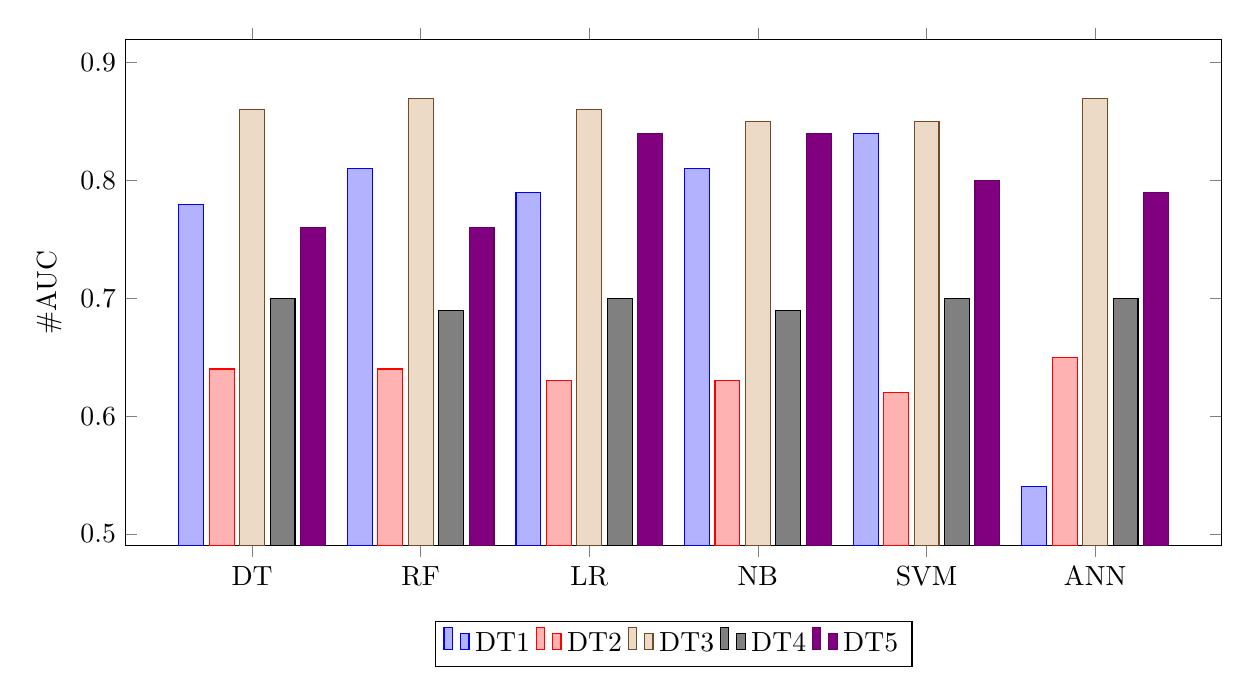
\begin{tikzpicture}
 \centering
\begin{axis}[
    height=8cm, width=15.5cm,
    bar width=0.4cm,
    ybar,
    %ybar=5pt,% configures `bar shift'
    bar width=9pt,
    enlargelimits=0.15,
    legend style={at={(0.5,-0.15)},
    anchor=north,legend columns=-1},
    ylabel={\#AUC},
    symbolic x coords={{DT,RF,LR,NB,SVM,ANN}},
    xtick=data,
    %nodes near coords,
    nodes near coords align={vertical},
    ]
\addplot coordinates {(DT,0.78) (RF, 0.81) (LR,0.79)(NB, 0.81)(SVM,0.84)(ANN, 0.54)};
\addplot coordinates{(DT,0.64) (RF, 0.64) (LR,0.63)(NB, 0.63)(SVM,0.62)(ANN, 0.65)};
\addplot coordinates {(DT,0.86) (RF, 0.87) (LR,0.86)(NB, 0.85)(SVM,0.85)(ANN, 0.87)};
\addplot coordinates {(DT,0.70) (RF, 0.69) (LR,0.70)(NB, 0.69)(SVM,0.70)(ANN, 0.70)};
\addplot coordinates {(DT,0.76) (RF, 0.76) (LR,0.84)(NB, 0.84)(SVM,0.80)(ANN, 0.79)};
\legend{DT1,DT2,DT3,DT4,DT5}
\end{axis}
\end{tikzpicture}
\caption{comparison of Roc Area achieved by six classifiers}
\end{figure}
However, on these same datasets, the algorithms often present very low specificities, for example 0.05 on DT1. This shows that our best performing classifiers are only able to predict a single class: either the patient has malaria or he does not, but not in both spots. This is because the DT1 and DT3 datasets are very unbalanced. In fact in these datasets either the number of patients with malaria is greater than those who are not or the opposite is true. Furthermore, we note that on the DT2 and DT4 datasets all the algorithms present specificities and Sensivity that are significant and quite similar. Contrary to what is quoted a little above, on these datasets the algorithms are efficient on the prediction tasks of the two classes. Looking closely at the results in terms of precision, recall and F-measure we observe that the classifiers RF, LR, SVM and ANN generally outperform the others for each dataset. Indeed, for the dataset DT1, which contains observations on patients living in different regions of Senegal, these four classifiers have an accuracy of 99\%, a recall greater than 92\% and an F-measure greater than 95\%. We note the same trend with the DT2 dataset which contains observations on patients living in the same area in Senegal. It can also be noted that RF, LR, SVM and ANN have better precision than the rapid diagnostic test carried out and systematically used in the majority of health structures in Senegal. This observation remains true with DT4 which is a perfectly balanced dataset. In conclusion, it is very difficult or even impossible for us to say definitively which algorithm is more efficient for the task of predicting malaria, but the choice of this one will strongly depend on the choice of the data set. However, this study shows that our classification problem has been taken care of. A method integrating several models and various datasets is necessary

\begin{figure}
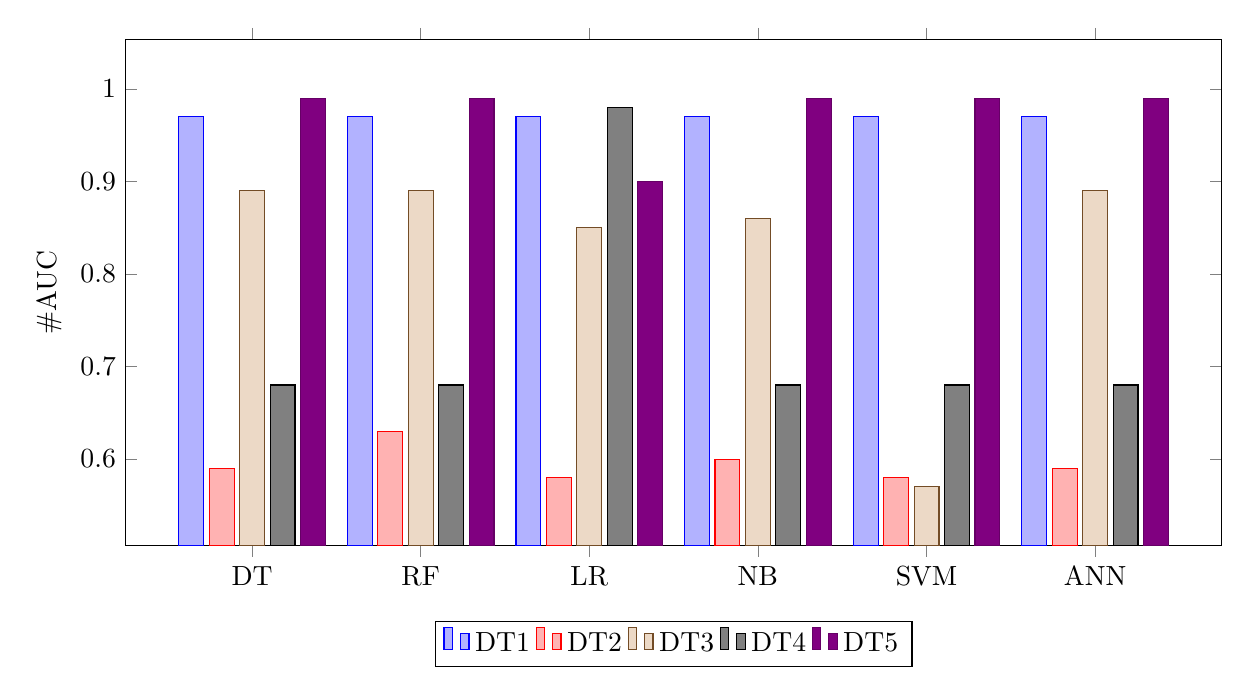
\begin{tikzpicture}
 \centering
\begin{axis}[
    height=8cm, width=15.5cm,
    bar width=0.4cm,
    ybar,
    %ybar=5pt,% configures `bar shift'
    bar width=9pt,
    enlargelimits=0.15,
    legend style={at={(0.5,-0.15)},
    anchor=north,legend columns=-1},
    ylabel={\#AUC},
    symbolic x coords={{DT,RF,LR,NB,SVM,ANN}},
    xtick=data,
    %nodes near coords,
    nodes near coords align={vertical},
    ]
\addplot coordinates {(DT,0.97) (RF, 0.97) (LR,0.97)(NB, 0.97)(SVM,0.97)(ANN, 0.97)};
\addplot coordinates{(DT,0.59) (RF, 0.63) (LR,0.58)(NB, 0.60)(SVM,0.58)(ANN, 0.59)};
\addplot coordinates {(DT,0.89) (RF, 0.89) (LR,0.85)(NB, 0.86)(SVM,0.57)(ANN, 0.89)};
\addplot coordinates {(DT,0.68) (RF, 0.68) (LR,0.98)(NB, 0.68)(SVM,0.68)(ANN, 0.68)};
\addplot coordinates {(DT,0.99) (RF, 0.99) (LR,0.90)(NB, 0.99)(SVM,0.99)(ANN, 0.99)};
\legend{DT1,DT2,DT3,DT4,DT5}
\end{axis}
\end{tikzpicture}
\caption{comparison of Precision achieved by six classifiers}

\end{figure}


\begin{figure}
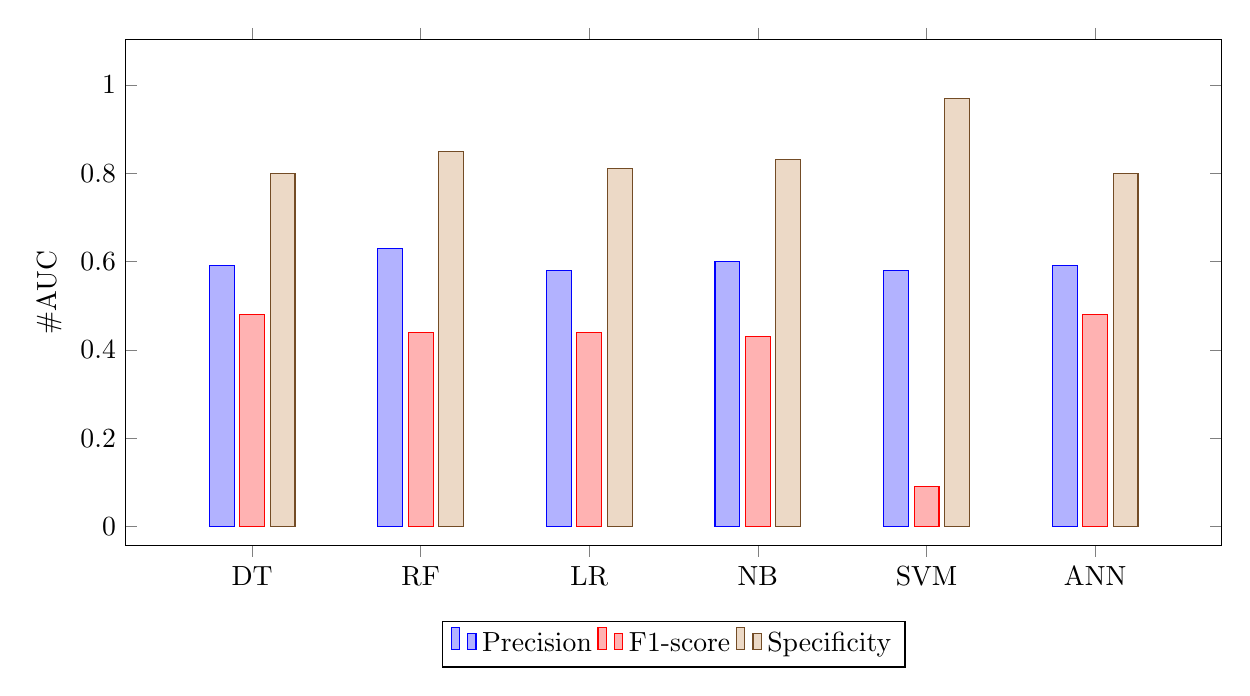
\begin{tikzpicture}
 \centering
\begin{axis}[
    height=8cm, width=15.5cm,
    bar width=0.4cm,
    ybar,
    %ybar=5pt,% configures `bar shift'
    bar width=9pt,
    enlargelimits=0.15,
    legend style={at={(0.5,-0.15)},
    anchor=north,legend columns=-1},
    ylabel={\#AUC},
    symbolic x coords={{DT,RF,LR,NB,SVM,ANN}},
    xtick=data,
    %nodes near coords,
    nodes near coords align={vertical},
    ]
\addplot coordinates {(DT,0.59) (RF, 0.63) (LR,0.58)(NB, 0.60)(SVM,0.58)(ANN, 0.59)};
\addplot coordinates{(DT,0.48) (RF, 0.44) (LR,0.44)(NB, 0.43)(SVM,0.09)(ANN, 0.48)};
\addplot coordinates {(DT,0.80) (RF, 0.85) (LR,0.81)(NB, 0.83)(SVM,0.97)(ANN, 0.80)};
%\addplot coordinates {(DT,0.68) (RF, 0.68) (LR,0.98)(NB, 0.68)(SVM,0.68)(ANN, 0.68)};
%\addplot coordinates {(DT,0.99) (RF, 0.99) (LR,0.90)(NB, 0.99)(SVM,0.99)(ANN, 0.99)};
\legend{Precision,F1-score,Specificity,DT4}
\end{axis}
\end{tikzpicture}
\caption{comparison of other performance measures in classifiers on DT1}

\end{figure}

% Conclusion
\section{Conclusion}\label{conclusion}
In this study, six ML models have been extensively tested and compared over various datasets in order to evaluate their performance for the task of predicting Malaria occurrence in a patient knowing his signs and symptoms. The results obtained show that some of them are promising and overcome RDT in particular settings. As future work, we plan to study the implementation of an ensemble method for predicting Malaria occurrence built on the algorithms offering the best performances in our present study. 

%
% ---- Bibliography ----
%
% BibTeX users should specify bibliography style 'splncs04'.
% References will then be sorted and formatted in the correct style.
%
\bibliographystyle{splncs04}
\bibliography{biblio}
%
\end{document}
